\documentclass[12pt]{report}

%-------------------------------------------------------
% THEMES, COLORS
%-------------------------------------------------------
\usepackage[top=2.5cm, bottom=3cm, left=2.5cm, right=2.5cm]{geometry}
\usepackage{amsmath,mathtools,bm,amsthm,amssymb}
\usepackage{underscore}
\usepackage{xcolor}
\usepackage{graphicx}
\usepackage{algpseudocode}

%--------------------------------------------------------
% COLOR DEFINITIONS
%---------------------------------------------------------
\definecolor{amber}{rgb}{1.0, 0.49, 0.0}
\definecolor{olivedrab}{rgb}{0.42, 0.56, 0.14}
\definecolor{darkolivegreen}{rgb}{0.33, 0.42, 0.18}
\definecolor{chromeyellow}{rgb}{1.0, 0.65, 0.0}
\definecolor{beige}{rgb}{0.96, 0.96, 0.86}
\definecolor{bluegreen}{rgb}{3, 166, 155}
\definecolor{pitchblack}{rgb}{0, 0, 0}
\definecolor{lightbeige}{rgb}{255, 251, 241}
\definecolor{mediumgray}{rgb}{183, 183, 183}
\definecolor{carrotorange}{rgb}{0.93, 0.57, 0.13}
\definecolor{orange-red}{rgb}{1.0, 0.27, 0.0}
\definecolor{ferngreen}{rgb}{0.31, 0.47, 0.26}
\definecolor{darkspringgreen}{rgb}{0.09, 0.45, 0.27}
\definecolor{cocoabrown}{rgb}{0.82, 0.41, 0.12}
\definecolor{darkorange}{rgb}{1.0, 0.55, 0.0}
\definecolor{deepcarrotorange}{rgb}{0.91, 0.41, 0.17}
%---------------------------------------------------------

%-------------------------------------------------------------------------
% NEW THEME
%-------------------------------------------------------------------------
\definecolor{UBCblue}{rgb}{0.04706, 0.13725, 0.26667} % UBC Blue (primary)
\definecolor{UBCgrey}{rgb}{0.3686, 0.5255, 0.6235} % UBC Grey (secondary)

%\usepackage{helvet}
%-------------------------------------------------------
% DEFFINING AND REDEFINING COMMANDS
%-------------------------------------------------------
\newcommand\var{\texttt}
\usepackage{amssymb}
\renewcommand{\emptyset}{\varnothing}
%-----------------------------------------------------------------------------
% FONTS TRIED
%-----------------------------------------------------------------------------
%\usepackage{ccfonts}
%\usepackage{mathpazo}
%\usepackage{newtxtext}
%\usepackage{newtxmath}
%% Times New Roman
%\setromanfont[
%BoldFont=timesbd.ttf,
%ItalicFont=timesi.ttf,
%BoldItalicFont=timesbi.ttf,
%]{times.ttf}
%% Arial
%\setsansfont[
%BoldFont=arialbd.ttf,
%ItalicFont=ariali.ttf,
%BoldItalicFont=arialbi.ttf
%]{arial.ttf}
%% Courier New
%\setmonofont[Scale=0.90,
%BoldFont=courbd.ttf,
%ItalicFont=couri.ttf,
%BoldItalicFont=courbi.ttf
%]{cour.ttf}
%-----------------------------------------------------------------------------
% FONT PACKAGES
%-----------------------------------------------------------------------------

\usepackage[utf8]{inputenc}
\usepackage[english]{babel}
\usepackage[T1]{fontenc}
\usepackage{fontspec}

\setmainfont{XCharter}
%\usepackage[libertine,cmintegrals,cmbraces,vvarbb]{newtxmath}
%\usepackage[scaled=0.95]{inconsolata}

%-------------------------------------------------------
% INFORMATION IN THE TITLE PAGE
%-------------------------------------------------------


\newtheorem{lemma}{Lemma}[chapter]
\newtheorem{theorem}{Theorem}[chapter]
\theoremstyle{definition}
\newtheorem{definition}{Definition}[chapter]
\newtheorem{example}{Example}[chapter]
\newtheorem*{note}{Note}
\newcommand{\samplecomp}{m_{\mathcal{H}}}
\newcommand{\SampleComp}[2]{m_{\mathcal{H}}(#1, #2)}
\newcommand{\usamplecomp}[2]{m_{\mathcal{H}}^{\text{UC}}(#1, #2)}
\newcommand{\USampleComp}{m_{\mathcal{H}}^{\text{UC}}}
\newcommand{\nusamplecomp}{\ensuremath{m_{\mathcal{H}}^{\text{NUL}}}}
\newcommand{\pacerror}[1]{L_{\mathcal{D}, f}(#1)}
\newcommand{\vcdim}{\ensuremath{\text{VCdim}}}
\newcommand{\algo}{\ensuremath{\mathcal{A}}}
\newcommand{\hypclass}{\ensuremath{\mathcal{H}}}
\newcommand{\parity}[1]{\ensuremath{\mathcal{H}_{#1\text{-parity}}}}
\newcommand{\rect}[1]{\ensuremath{\mathcal{H}_{\text{rect}}^{#1}}}
\newcommand{\conj}[1]{\ensuremath{\mathcal{H}_{\text{con}}^{#1}}}
\newcommand{\mconj}[1]{\ensuremath{\mathcal{H}_{\text{mcon}}^{#1}}}
\newcommand{\zeroone}{\ensuremath{\operatorname{0-1}}}
\newcommand{\dom}{\ensuremath{\mathcal{X}}}
\newcommand{\range}{\ensuremath{\mathcal{Y}}}
\newcommand{\Nat}{\ensuremath{\mathbf{N}}}
\newcommand{\dist}{\ensuremath{\mathcal{D}}}
\newcommand{\R}{\ensuremath{\mathbf{R}}}
\newcommand{\Rone}{\ensuremath{\mathbf{R}}}
\newcommand{\Rpos}{\ensuremath{\mathbf{R}_{+}}}
\newcommand{\Rtwo}{\ensuremath{\mathbf{R}^2}}
\newcommand{\Prtwo}[2]{\mathbf{Pr}_{#1} \left \{ #2 \right \}}
\newcommand{\Prone}[1]{\mathbf{Pr} \left \{ #1 \right \}}
\newcommand{\Exptwo}[2]{\mathbf{E}_{#1} \left [ #2 \right ]}
\newcommand{\Expone}[1]{\mathbf{E} \left [ #1 \right ]}
\newcommand{\ceiling}[1]{\ensuremath{\left \lceil #1 \right \rceil}}
\newcommand{\angular}[1]{\ensuremath{\left \langle #1 \right \rangle}}
\newcommand{\floor}[1]{\ensuremath{\left \lfloor #1 \right \rfloor}}
\newcommand{\dx}{\ensuremath{\text{d}}}
\newcommand{\ind}{\ensuremath{\mathbf{1}}}
\newcommand{\Mod}[1]{\ (\mathrm{mod}\ #1)}
\newcommand{\basisvec}{\ensuremath{\boldsymbol{e}}}
\newcommand{\vect}[1]{\ensuremath{\boldsymbol{#1}}}
\newcommand{\trans}[1]{\ensuremath{#1}^{\intercal}}

\DeclareMathOperator{\ERM}{ERM}
\DeclareMathOperator{\pos}{POS}
\DeclareMathOperator{\HS}{HS}
\DeclareMathOperator{\HHS}{HHS}
\DeclareMathOperator{\id}{id}
\DeclareMathOperator{\sign}{sign}
\DeclarePairedDelimiter\norm{\lVert}{\rVert}

\newtheorem{exercise}{Exercise}

\newenvironment{solution}
  {\renewcommand\qedsymbol{$\blacksquare$}\begin{proof}[Solution]}
  {\end{proof}}

\title{Neural Networks and Deep Learning: Exercises}

\author{Somnath Sikdar}
\date{\today}

\begin{document}
\maketitle
\tableofcontents

\chapter{Markov Decision Processes}

\section{Introduction}
Reinforcement learning consists in teaching an agent how to behave using 
observations from its environment with the goal of maximizing 
future rewards that it receives in response to its behavior. 
The set-up consists of an \emph{agent}, 
which is the learner or decision maker and the \emph{enviroment}, which is 
the thing that the agent interacts with, comprising everything outside the agent. 
The agent and the environment interact in discrete time steps. At a given time 
step~$t$, the agent takes an \emph{action} and the environment responds by 
presenting a new state and a scalar feedback signal called the \emph{reward}.

\begin{figure}[h]
\begin{center}
    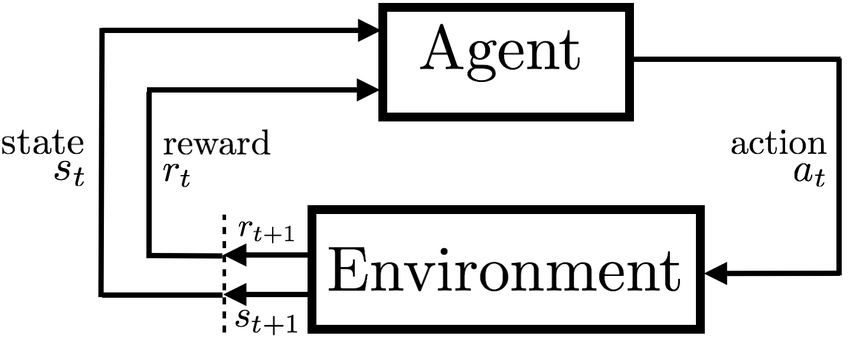
\includegraphics[scale=0.3]{RLAgentEnvironment.png}
\end{center}   
\caption{The agent and the environment}
\end{figure}


Problems in reinforcement learning are typically formulated in the formal
setting of a Markov Decision Process (MDP). An MDP is a five-tuple
$\angular{\states, \actions, p, \rewards, \discount}$
\begin{itemize}
    \item a set $\states$ of states
    \item a set $\actions$ of actions
    \item a set $\rewards$ of rewards
    \item a probability function
        $p \colon \states \times \rewards \times \states \times \actions \rightarrow [0, 1]$
    \item a discount factor $\discount \in [0, 1]$
\end{itemize}

The probablity function~$p$ defines the dynamics of the MDP. It tells us what 
the most likely next state and reward combination are given the current state 
and the action taken by the agent. 
\begin{equation}
    p(s', r \mid s, a) \defn \Prone{S_{t + 1} = s', R_{t + 1} = r \mid S_t = s, A_t = a}.
\end{equation} 
In the above equation, we assume that the probability does \emph{not} depend 
on the time step~$t$. Such an MDP is called \emph{stationary}. 
Since this is a probablity distribution, for all $s \in \states$ and for all 
$a \in \actions$,
\begin{equation}
    \sum_{s' \in \states} \sum_{r \in \rewards} p(s', r \mid s, a) = 1.
\end{equation}
We also define a state-transition probability function 
$p \colon \states \times \actions \times \states \rightarrow [0, 1]$ defined as:
\begin{equation}
    p(s' \mid s, a) \defn \sum_{r \in \rewards}  p(s', r \mid s, a).
\end{equation}

In response to the action taken by the agent, the environment provides it a 
scalar rewards at each time step. The total reward of the agent in time step $t$ is
defined as
\begin{equation}
    G_t \defn \sum_{k = 0}^{\infty} R_{t + k + 1}.
\end{equation}
With infinite time horizons, this reward could go to infinity. To prevent this,
one uses a discounting factor $\gamma \in [0, 1]$ and defines the total reward as
\begin{equation}
    G_t \defn R_{t + 1} + \gamma \cdot R_{t + 2} + \gamma^2 \cdot R_{t + 3} + \cdots 
\end{equation}

\subsection{Policy and Value Functions}
A \emph{policy}~$\policy$ is a mapping from states to probabilities of selecting each possible 
action. 
\begin{equation}
    \policy (a \mid s) \defn \Prone {A_t = a \mid S_t = s}.
\end{equation}
Note that this probability distribution does not depend on the time step~$t$.

\begin{exer}
If the current state is $S_t$, and actions are selected according to a stochastic
policy $\policy$, then what is the expectation of $R_{t + 1}$ in terms of 
$\policy$ and the four-argument function~$p$?
\end{exer}
\begin{solution}
Let us assume that the current state $S_t = s$. We may write 
$\Exptwo{\policy}{R_{t + 1} \mid S_t = s}$ as:
\begin{align*}
    \Exptwo{\policy}{R_{t + 1} \mid S_t = s} 
        & = \sum_{r \in \rewards} r \cdot \Prtwo{\policy}{R_{t + 1} = r \mid S_t = s} \\
        & = \sum_{r \in \rewards} r \cdot \sum_{a \in \actions} 
                \Prtwo{\policy}{R_{t + 1} = r\mid S_t = s, A_t = a} 
                    \cdot \Prtwo{\policy}{A_{t} = a \mid S_t = s} \\ 
        & = \sum_{r \in \rewards} r \cdot \sum_{a \in \actions} 
            \sum_{s' \in \states} p(s', r \mid s, r) \cdot \policy (a \mid s) 
\end{align*}
\qed
\end{solution}

The \emph{value function} of a state~$s$ under a policy~$\policy$, denoted 
$v_{\policy}(s)$, is the expected return when starting in state~$s$ and 
following $\policy$ thereafter. For an MDP, we may write the value function as:
\begin{equation}
    v_{\policy}(s) \defn \Exptwo{\policy}{G_t \mid S_t = s} 
        = \Exptwo{\policy}{\sum_{k = 0}^{\infty} \discount^{k} \cdot R_{t + k + 1} \bigm\vert S_t = s }.
\end{equation}
The function $v_{\policy}(s)$ is called the \emph{state-value function} of the policy $\policy$.

We also define the value of taking an action $a$ in state $s$ under a policy $\policy$, 
denoted $q_{\policy}(s, a)$, as the expected return when starting in state $s$, 
taking action $a$ and following $\policy$ thereafter.
\begin{equation}
    q_{\policy}(s, a) \defn \Exptwo{\policy}{G_t \mid S_t = s, A_t = a} 
        = \Exptwo{\policy}{\sum_{k = 0}^{\infty} \discount^{k} \cdot R_{t + k + 1} \bigm\vert S_t = s, A_t = a}.
\end{equation}
The function $q_{\policy}(s, a)$ is the \emph{action-value function} of the policy~$\policy$. 

\begin{exer}
Give an equation for $v_{\policy}$ in terms of $q_{\policy}$ and $\policy$.
\end{exer}
\begin{solution}
We may write $v_{\policy}(s)$ as:
\begin{align*}
    v_{\policy}(s) & \defn \Exptwo{\policy}{G_t \vert S_t = s} \\
                   & = \sum_{a \in \actions} \Exptwo{\policy}{G_t \vert S_t = s, A_t = a} 
                        \cdot \Prtwo{\policy}{A_t = a \vert S_t = a} \\
                   & = \sum_{a \in \actions} q_{\policy}(s, a) \policy (a \vert s).
\end{align*}
\qed
\end{solution}

\begin{exer}
Give an equation for $q_{\policy} (s, a)$ in terms of $v_{\policy}$ and the 
four parameter function~$p$. 
\end{exer}
\begin{solution}
\begin{align*}
    q_{\pi}(s, a) & \defn \Exptwo{\policy}{R_{t + 1} + \discount \cdot R_{t + 2} + \discount^2 \cdot R_{t + 3} + \cdots \vert S_t = s, A_t = a} \\
                  & = \Exptwo{\policy}{R_{t + 1} \vert S_t = s, A_t = a} + 
                    \discount \cdot \Exptwo{\policy}{G_{t + 1} \vert S_t = s, A_t = a} \\
                  & = \sum_{r \in \rewards} r \cdot \Prtwo{\policy}{R_{t + 1} = r \vert S_t = s, A_t = a} + \\
                  & \quad \quad \discount \cdot \sum_{s' \in \states} \Exptwo{\policy}{G_{t + 1} \vert S_{t + 1} = s', S_t = s, A_t = a}
                        \cdot \Prtwo{\policy}{S_{t + 1} = s' \vert S_t = s, A_t = a} \\ 
                  & = \sum_{r \in \rewards} r \cdot \sum_{s' \in \states} p(s', r \vert s, a) + 
                    \discount \cdot \sum_{s' \in \states} \Exptwo{\policy}{G_{t + 1} \vert S_{t + 1} = s'} 
                        \cdot \sum_{r \in \rewards} p(s', r \vert s, a) \\
                  & = \sum_{r \in \rewards} \sum_{s' \in \states} \left [ r + \discount \cdot v_{\policy}(s') \right ] p(s', r \vert s, a).
\end{align*}
\end{solution}

Based on the last two exercises, we may write:
\begin{equation}
    v_{\policy} (s) = \sum_{a \in \actions} \policy (a \vert s) \cdot 
            \sum_{r \in \rewards} \sum_{s' \in \states} \left [ r + \discount \cdot v_{\policy}(s') \right ] p(s', r \vert s, a).
\end{equation}

\chapter{The Backpropagation Algorithm}

\section{The Backpropagation Equations}

Before we describe anything, we briefly recap notation. We let
$C$ denote the cost function and $\sigma$ the activation function
of the neurons.
\begin{enumerate}
    \item $w_{j k}^{l}$ is the weight of the link between the $j$th
        neuron in layer~$l$ and the $k$th neuron in layer~$l - 1$.
    \item $b_j^l$ is the bias of neuron $j$ in layer~$l$.
    \item $z_{j}^l$ is the weighted input to neuron~$j$ in layer~$l$.
    \item $a_j^{l} = \sigma(z_{j}^l)$ is the activation of neuron~$j$ in
        layer~$l$.
    \item $\delta_{j}^{l} := \partial C / \partial z_{j}^{l}$ is
        the ``error'' of neuron~$j$ in layer~$l$.
\end{enumerate}

Using this notation, we may write the weighted output to neuron~$j$
in the $l$th layer as:
\[
    z_{j}^{l} = \sum_{k} w_{j k}^l a_{k}^{l - 1} + b_{j}^l =
                \sum_{k} w_{j k}^l \sigma (z_{k}^{l - 1}) + b_{j}^l,
\]
where the index~$k$ runs over all neurons in layer~$l - 1$ and
$2 \leq l \leq L$. Symbols such as $w^{l}$, $b^{l}$, $a^{l}$ without
subscripts refer to either matrices or vectors as the case may be.
For example, $w^{l}$ refers to the matrix whose $(j, k)$th element
is $w_{j k}^{l}$. This matrix has as many rows as there are neurons
in the $l$th layer and as many columns as there are neurons in
layer~$l - 1$. The symbol~$b^{l}$ refers to the vector of
biases~$b_{j}^l$ of the neurons in layer~$l$; similarly, $a^{l}$
refers to the vector of activations~$a_{j}^l$ of the neurons in
layer~$l$.

To understand why it makes sense to call
$\delta_{j}^{l} := \partial C / \partial z_{j}^{l}$  the ``error,'' consider a
small change $\Delta z_j^l$ in $z_j^l$. Then the change in the cost function $C$
as a result of this change in $z_j^l$ is $\partial C / \partial z_j^l \cdot \Delta z_j^l$.
If $\partial C / \partial z_{j}^{l} > 0$, then the cost increases as we increase
$\Delta z_j^l$; thus to reduce the cost, we must choose $\Delta z_j^l < 0$. Similarly,
if $\partial C / \partial z_{j}^{l} < 0$, then the cost increases if $\Delta z_j^l < 0$
and in order to reduce cost, we should select $\Delta z_j^l > 0$. Finally, if
$\partial C / \partial z_{j}^{l} \approx 0$, then changes in $z_j^l$ do not
affect the final cost. Thus $\partial C / \partial z_{j}^{l}$ indicates how we
should change the input $z_j^l$ to the $j$th neuron in layer~$l$.

We will derive the complete set of backpropagation equations in four steps.

With this notation in hand, we may write the backpropagation equations
as:
\begin{equation}
\boxed{
\setlength{\jot}{12pt}
\begin{aligned}
    \delta^{L} & = \nabla_{a^L} C \odot \sigma'(z^L) \\
    \delta^{l} & = ( \trans{(w^{l + 1})} \delta^{l + 1} ) \odot \sigma'(z^l) \\
    \frac{\partial C}{\partial b_j^{l}} & = \delta_{j}^l := \frac{\partial C}{\partial z_j^l}\\
    \frac{\partial C}{\partial w_{j k}^l} & = a_{k}^{l - 1} \delta_{j}^l
\end{aligned}
}
\end{equation}

\section{Backpropagation Applied to Gradient Descent}

The backpropagation procedure calculates the gradient of the cost
function~$C$ with respect to a single input example. To make use of
backprop in the context of stochastic gradient descent, we need to take
the mean of the gradient computed over all examples in a mini batch.
Let's suppose that we have a mini batch with $m$ examples
$x_1, \ldots, x_m$.
\begin{enumerate}
    \item For each training example~$x$, set the input activation
        $a^1 (x)$ and perform the following steps:
        \begin{enumerate}
            \item \textbf{Feedforward.} For $2 \leq l \leq L$, set
                $z^l (x) = w^l a^{l - 1} (x) + b^l$ and
                $a^l (x) = \sigma (z^l (x))$.
            \item \textbf{Output Error.} Calculate
                $\delta^L (x) = \nabla_{a^L} C(x) \odot \sigma' (z^L (x) )$.
            \item \textbf{Backprop.} For $L - 1 \leq l \leq 2$,
                $\delta^l (x) = ( \trans{(w^{l + 1})} \delta^{l + 1} (x) )
                                    \odot \sigma' (z^l (x))$.
            \item \textbf{Gradients.} Calculate
            $ \frac{\partial C}{\partial b_j^{l}} (x) = \delta_{j}^l (x)$
            and $\frac{\partial C}{\partial w_{j k}^l} (x)
                    = a_{k}^{l - 1} \delta_{j}^l (x)$.
        \end{enumerate}
    \item \textbf{Gradient Descent.} For $L \leq l \leq 2$, set
        $w^l = w^l - \frac{\eta}{m} \sum_{x} \delta^{l} (x) \trans{(a^{l - 1} (x))}$
        and
        $b^l = b^l - \frac{\eta}{m} \sum_{x} \delta^l (x)$.
\end{enumerate}

\end{document}

